\chapter{Feature Detection and Tracking}
\label{ch:frontend}

\begin{objectives}
\begin{itemize}
  \item Derive the structure tensor from the auto-correlation of an image patch, and understand corner detectors (Harris, Shi--Tomasi, FAST).
  \item Derive Lucas--Kanade optical flow from brightness constancy, as a Gauss--Newton problem, including the aperture problem.
  \item Implement iterative, pyramidal Lucas--Kanade tracking, and know its failure modes.
  \item Build a robust tracking pipeline: bucketing, forward-backward checks, IMU-aided prediction and geometric verification.
  \item Manage feature tracks through their life cycle with bounded memory.
\end{itemize}
\end{objectives}

The front end turns a stream of images into \emph{feature tracks}: for each tracked scene point, the list of its undistorted normalized coordinates in the images
where it was seen, with the image timestamps. Everything the MSCKF knows about the scene comes from these tracks, so their quality bounds the quality of the
estimator.

\begin{figure}[h]
\centering
\begin{tikzpicture}[node distance=4mm and 5mm, every node/.style={block, font=\footnotesize, minimum width=19mm}]
  \node (img) {image $k$};
  \node (pyr) [right=of img] {build\\pyramid};
  \node (lk) [right=of pyr] {track with\\pyramidal LK};
  \node (fb) [right=of lk] {forward-\\backward check};
  \node (und) [below=of fb] {undistort\\points};
  \node (ran) [left=of und] {RANSAC\\(E or 2-pt)};
  \node (det) [left=of ran] {detect new\\corners (grid)};
  \node (out) [left=of det, fill=white] {tracks to\\estimator};
  \draw[->] (img) -- (pyr); \draw[->] (pyr) -- (lk); \draw[->] (lk) -- (fb);
  \draw[->] (fb) -- (und); \draw[->] (und) -- (ran); \draw[->] (ran) -- (det); \draw[->] (det) -- (out);
\end{tikzpicture}
\caption{A KLT-based front end, as used by MSCKF-style estimators.}
\label{fig:frontend-pipeline}
\end{figure}

% ==============================================================================
\section{What makes a good feature}

\subsection{The auto-correlation of a patch}

A feature is useful if it can be found again, precisely, in the next image. Consider a small window $W$ around a point and ask how much the window changes when
shifted by a small displacement $d$. Measure the change by the weighted sum of squared differences
\begin{equation}
  E(d) = \sum_{x\in W}w(x)\,\big(I(x + d) - I(x)\big)^2,
\end{equation}
with a window function $w$ (uniform, or a Gaussian that emphasizes the center). By a first-order Taylor expansion $I(x + d) \approx I(x) + \nabla I(x)\T d$, so
\begin{equation}
  E(d) \approx \sum_{x\in W}w(x)\,\big(\nabla I(x)\T d\big)^2 = d\T M\,d,
  \qquad
  M = \sum_{x\in W}w(x)\begin{bmatrix} I_u^2 & I_uI_v \\ I_uI_v & I_v^2 \end{bmatrix},
  \label{eq:structure-tensor}
\end{equation}
with the gradients $I_u$, $I_v$ computed as in \cref{sec:image-derivatives}. $M$ is the \term{structure tensor} (second-moment matrix) of the window: a symmetric PSD
$2\times2$ matrix, so $E(d)$ is a quadratic form whose level sets are ellipses (\cref{fig:ellipse}). Its eigenvalues $\lambda_1 \ge \lambda_2 \ge 0$ describe how distinctive the
window is.
\begin{itemize}
  \item Both small: the window is \emph{flat}; it looks the same after any small shift.
  \item One large, one small: an \emph{edge}; shifting along the edge (the eigenvector of $\lambda_2$) changes nothing.
  \item Both large: a \emph{corner}; every shift changes the window, so its position is well defined in two dimensions.
\end{itemize}
By the Rayleigh quotient (\cref{prop:rayleigh}), $\lambda_2$ is the smallest change $E(d)$ caused by any unit shift: the worst-case distinctiveness.

\subsection{Corner detectors}

\index{Harris detector}\index{Shi--Tomasi detector}
The \term{Harris detector}~\cite{harris1988corner} scores each pixel with $\det M - k(\tr M)^2 = \lambda_1\lambda_2 - k(\lambda_1 + \lambda_2)^2$, with $k \approx 0.04$--$0.06$, which avoids computing
eigenvalues. The \term{Shi--Tomasi detector}~\cite{shi1994good} scores $\lambda_2 = \min(\lambda_1, \lambda_2)$ directly (\cref{fig:structure-tensor}), computed in closed form for a $2\times2$
matrix as $\tfrac12\big(\tr M - \sqrt{(\tr M)^2 - 4\det M}\big)$. Both are followed by thresholding and non-maximum suppression. Shi--Tomasi has a deeper justification: it
selects exactly the windows for which the tracker of the next section is well conditioned.

\begin{figure}[t]
  \centering
  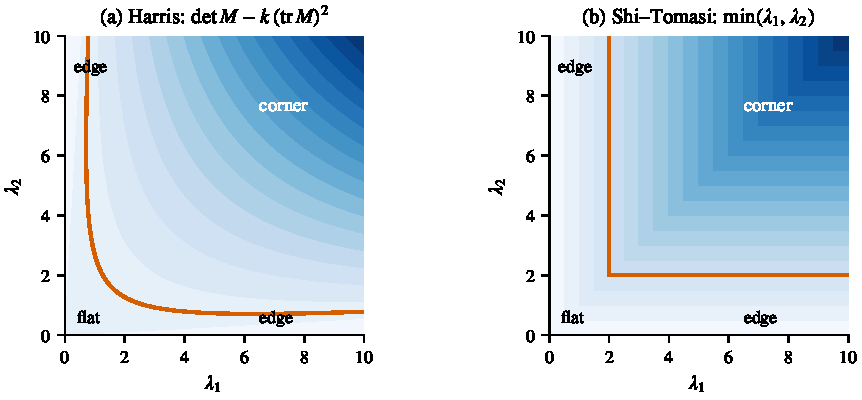
\includegraphics[width=\textwidth]{fig_structure_tensor.pdf}
  \caption{Corner scores over the plane of structure-tensor eigenvalues, with a threshold contour (orange). Both scores accept only windows with two large
  eigenvalues. Shi--Tomasi's $\min(\lambda_1, \lambda_2)$ is exactly the quantity that makes the Lucas--Kanade system well conditioned.}
  \label{fig:structure-tensor}
\end{figure}

\begin{figure}[t]
  \centering
  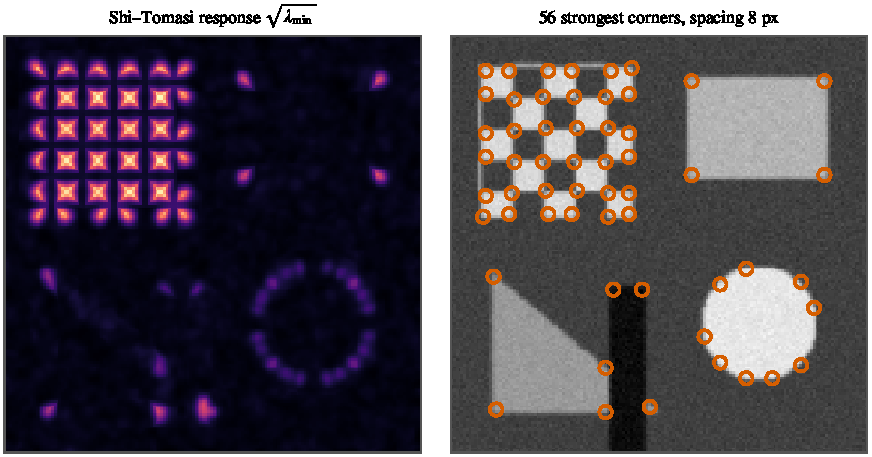
\includegraphics[width=\textwidth]{fig_harris.pdf}
  \caption{Shi--Tomasi corner response on a synthetic image (left), and the strongest corners after non-maximum suppression with a minimum spacing of 8~px (right).
  Edges and flat regions get low scores; corners and blob-like texture get high ones.}
  \label{fig:harris}
\end{figure}

Other detectors trade quality for speed. FAST classifies a pixel as a corner if a long enough arc of the 16 pixels on a circle around it is uniformly brighter or
darker than the center, using only comparisons; it is very fast but noisier. Detectors used for matching across large viewpoint changes add \emph{scale}
selection (detecting at several pyramid levels) and an \emph{orientation} for each feature, as ORB does. A frame-to-frame tracker needs neither.

% ==============================================================================
\section{Lucas--Kanade optical flow}

\subsection{Brightness constancy and the aperture problem}

Assume that a scene point keeps its brightness between consecutive frames, $I_{k+1}(x + d) = I_k(x)$, where $d$ is the image motion of the point. Linearizing in $d$,
\begin{equation}
  I_{k+1}(x) + \nabla I\T d \approx I_k(x)
  \quad\Longleftrightarrow\quad
  I_u\,d_u + I_v\,d_v + I_t = 0, \qquad I_t = I_{k+1}(x) - I_k(x).
  \label{eq:ofc}
\end{equation}
This \emph{optical-flow constraint} is one equation in two unknowns. It determines only the component of $d$ along the gradient: motion along an edge is invisible.
This is the \term{aperture problem}, the same phenomenon seen through a small hole when a long line slides past: only its perpendicular motion is visible.

\subsection{The Lucas--Kanade solution}

\index{Lucas--Kanade tracker}
Lucas and Kanade~\cite{lucas1981iterative} assume the displacement is the same for all pixels of a small window, which provides many equations for the two
unknowns, and solve \eqref{eq:ofc} for all of them in the least-squares sense:
\begin{equation}
  \min_d \sum_{x\in W}w(x)\big(\nabla I(x)\T d + I_t(x)\big)^2
  \quad\Longrightarrow\quad
  M\,d = -\sum_{x\in W}w(x)\,I_t(x)\,\nabla I(x),
  \label{eq:lk}
\end{equation}
with the structure tensor $M$ of \eqref{eq:structure-tensor} as the normal matrix (\cref{sec:least-squares}). The system is solvable and well conditioned exactly when both
eigenvalues of $M$ are large compared with the image noise: Shi and Tomasi's insight was to select features by the very criterion that makes them trackable. With
image noise of variance $\sigma_I^2$ per pixel, the covariance of the estimated displacement is approximately $\sigma_I^2M\inv$ (\cref{prop:wls-cov}), so $1/\sqrt{\lambda_2}$ measures
how precisely the worst direction is tracked.

\subsection{Iterative refinement}

\Cref{eq:lk} rests on a linearization that holds only for small $d$. The full problem, minimizing $\sum_xw(x)(I_{k+1}(x + d) - I_k(x))^2$ over $d$, is a nonlinear least-squares
problem, and Lucas--Kanade is its Gauss--Newton solution (\cref{ch:nlls}):

\begin{algorithm}[h]
\caption{Iterative Lucas--Kanade for one feature}
\label{alg:lk}
\begin{algorithmic}[1]
\Require images $I_k$, $I_{k+1}$; feature position $x_0$; initial guess $d$ (zero, or a prediction)
\State compute the template $T(x) = I_k(x)$ and its gradients over the window around $x_0$; compute $M$ and factor it
\Repeat
  \State sample $I_{k+1}(x + d)$ over the window with bilinear interpolation (\cref{sec:interpolation})
  \State $e(x) \gets I_{k+1}(x + d) - T(x)$ \Comment{residual image}
  \State solve $M\,\Delta d = -\sum_xw(x)\,e(x)\,\nabla T(x)$
  \State $d \gets d + \Delta d$
\Until{$\|\Delta d\| < 0.01$~px or the iteration limit is reached}
\end{algorithmic}
\end{algorithm}

Using the gradients of the \emph{template} $T = I_k$ rather than of the warped image lets $M$ be computed and factored once per feature (the \emph{inverse
compositional} idea, analyzed by Baker and Matthews~\cite{baker2004lk}). Sub-pixel accuracy comes from the bilinear interpolation. A few iterations usually
suffice when the initial guess is within the window radius.

\subsection{Pyramids}

The linearization is valid only for displacements smaller than the scale over which the image gradient is roughly constant, about the window radius. Fast motion
violates this: at 1~rad/s and 20~Hz, the image moves by about 23~px between frames. The remedy is a Gaussian pyramid (\cref{sec:pyramids}). Tracking starts at the
coarsest level, where a 24-pixel motion becomes a 3-pixel motion; the result, doubled, initializes the next finer level, and so on down to full resolution
(\cref{fig:pyramid})~\cite{bouguet2001pyramidal}. With $L$ levels above the base, the trackable displacement grows by about $2^L$.

\begin{figure}[t]
\centering
\begin{tikzpicture}[scale=0.9]
  \foreach \l/\s/\y in {0/3.2/0, 1/1.6/2.0, 2/0.8/3.2, 3/0.4/3.95} {
    \draw[fill=primarylight, draw=primary] (-\s, \y) -- (\s, \y) -- ({\s*0.75}, {\y + 0.35}) -- ({-\s*0.75}, {\y + 0.35}) -- cycle;
    \node[font=\footnotesize, right] at ({\s + 0.2}, {\y + 0.15}) {level \l: $\frac{1}{2^{\l}}$ resolution};
  }
  \draw[->, plotorange, thick] (-0.3,4.2) -- (-0.15,3.55) -- (0.2,2.4) -- (0.9,0.25);
  \node[plotorange, font=\footnotesize, align=right, left] at (-2.0,3.2) {coarse estimate,\\refined at each level};
\end{tikzpicture}
\caption{Pyramidal tracking. A displacement that is too large to linearize at full resolution is small at the top level; each level doubles the estimate and refines
it.}
\label{fig:pyramid}
\end{figure}

\begin{figure}[t]
  \centering
  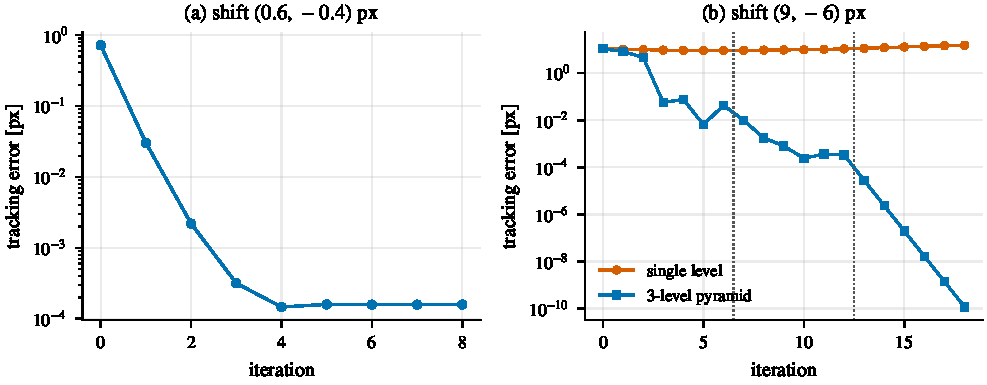
\includegraphics[width=\textwidth]{fig_lk.pdf}
  \caption{Lucas--Kanade on a synthetic textured image. (a) For a small shift of $(0.6, -0.4)$~px, the tracking error falls by orders of magnitude in a few
  Gauss--Newton iterations. (b) For a shift of $(9, -6)$~px, single-level tracking stalls in a wrong local minimum, while a three-level pyramid converges.}
  \label{fig:lk}
\end{figure}

\subsection{When tracking fails}

Lucas--Kanade fails when its assumptions fail: on edges and flat regions (an ill-conditioned $M$, the aperture problem); under occlusion, when the point disappears
behind another object; under strong brightness changes (\cref{ch:imageproc}); under motion blur, which smears the texture the tracker relies on; and when the
window straddles a depth discontinuity, where the two halves move differently. Most failures go undetected by the tracker itself, which returns a confident but wrong
position. Hence the checks of the next section.

% ==============================================================================
\section{Making tracking robust}

Optical flow optimizes photometric similarity, not physical correctness. It will track the shadow of a moving object, a specular highlight, or a T-junction formed by
two objects at different depths. Several layers of checks remove such tracks.
\begin{enumerate}
  \item \textbf{Forward-backward consistency.} Track each point from frame $k$ to $k+1$, then back to $k$. A correct track returns to its starting point; reject it if
        the round-trip error exceeds a fraction of a pixel.
  \item \textbf{IMU-aided prediction.} The gyroscope predicts the rotation between frames, $R_{c_2c_1} = R_{bc}\T R_{b_1b_2}\T R_{bc}$, where $R_{b_1b_2}$ is the integrated gyro rotation.
        For distant points, or a purely rotating camera, image points move by the infinite homography (\cref{ch:camera}): in pixels,
        $\tilde u_2 \propto KR_{c_2c_1}K\inv\tilde u_1$ (after undistortion). Starting LK from this prediction gives it a much better initial guess, and allows smaller windows and
        fewer pyramid levels.
  \item \textbf{Geometric verification.} Reject tracks that violate the epipolar constraint, with essential-matrix or two-point RANSAC, or the rotation-only constraint under
        low parallax (\cref{ch:multiview}).
  \item \textbf{Statistical gating in the filter.} Tracks that pass all of the above are still gated by the $\chi^2$ test of the MSCKF update (\cref{ch:msckfupdate}).
\end{enumerate}

\subsection{Feature distribution}

Asking a detector for the 200 strongest corners typically returns clusters on the most textured object in view. Clustered features constrain the motion poorly:
features in a small patch of the image make rotation and translation hard to separate. The standard remedy is \emph{grid bucketing}: divide the image into cells
(for example $8\times6$) and cap the number of features per cell, plus a minimum distance between features. New features are detected only in cells that have fallen
below their quota, using a mask around existing tracks. A uniform distribution of bearings makes the stacked measurement Jacobian better conditioned, which is
exactly what the estimator needs.

% ==============================================================================
\section{The feature life cycle}

\begin{figure}[h]
\centering
\begin{tikzpicture}[node distance=13mm and 34mm, every node/.style={font=\small}]
  \node[block] (new) {NEW};
  \node[block, right=of new] (trk) {TRACKED};
  \node[block, right=of trk] (lost) {LOST};
  \node[block, below=of trk, fill=white] (used) {consumed by update\\or discarded};
  \draw[->, thick] (new) -- node[above, font=\footnotesize]{tracked} (trk);
  \draw[->, thick] (trk) edge[loop above] node[above, font=\footnotesize]{tracked again} (trk);
  \draw[->, thick] (trk) -- node[above, font=\footnotesize]{track fails} (lost);
  \draw[->, thick] (lost) |- (used);
  \draw[->, thick] (trk) -- node[right, font=\footnotesize, align=left]{oldest observation's\\clone leaving the window} (used);
  \draw[->, thick] (new) |- node[left, font=\footnotesize, pos=0.25]{rejected} (used);
\end{tikzpicture}
\caption{Feature life cycle. A track is handed to the MSCKF update when it is lost, or when its oldest observation is about to leave the sliding window
(AGENTS.md F5). Its observations are used once and then discarded.}
\label{fig:lifecycle}
\end{figure}

Each feature has a persistent ID and a history of observations: (clone index or image timestamp, normalized coordinates). Since the estimator can only use
observations made at times that still have a clone in the window, the history never needs to exceed \code{kMaxClones} entries. That makes it possible to store all
tracks in a fixed-capacity pool with fixed-capacity histories, so the steady state of the front end performs no allocation for its bookkeeping (Milestone 9).

\begin{pitfall}[using a measurement twice]
Once a track's observations have been used in an MSCKF update, they must never be used again, not even partially. Re-using them double counts the same information
and makes the filter overconfident. If a track continues after being used (because its oldest clone was marginalized), its subsequent observations start a fresh
track.
\end{pitfall}

% ==============================================================================
\section{Engineering the front end}

The front end is the one component allowed to allocate (AGENTS.md E4), because OpenCV allocates internally, but it must reuse its buffers. In practice: keep the
previous pyramid and swap it with the new one instead of rebuilding storage; preallocate point vectors with \code{reserve}; keep the \code{cv::Mat} objects as members
so that their memory is reused when sizes do not change; and \emph{measure} the remaining allocations with the allocation guard rather than claiming they are zero.
Feature tracking is typically the most expensive part of the pipeline in time, too, so bucketing parameters, window size and pyramid depth are the main
performance knobs.

Descriptor-based front ends (ORB, BRIEF) describe each feature by a binary string of intensity comparisons in its neighborhood and match features across frames by
the Hamming distance between descriptors, rejecting ambiguous matches whose best and second-best distances are similar (the \emph{ratio test}). They handle large
viewpoint changes and re-detection after occlusion, which matters for loop closure, but for frame-to-frame VIO at 20~Hz KLT tracking is cheaper and more accurate.
Direct methods skip features altogether and use photometric error in the estimator itself.

\begin{projectlink}[Milestones 8 and 9]
M8 builds detection, bucketing, pyramidal LK with forward-backward checks, persistent IDs and point undistortion, and tests them on synthetic images with known
sub-pixel motion. M9 adds the life-cycle manager with a fixed-capacity pool and essential-matrix RANSAC in normalized coordinates, including the documented
pure-rotation behavior.
\end{projectlink}

\begin{takeaways}
\begin{itemize}
  \item The structure tensor $M$, from a first-order expansion of the patch auto-correlation, measures how well a window's position is defined; corners have two
        large eigenvalues.
  \item Lucas--Kanade is Gauss--Newton on the patch alignment error; its normal matrix is $M$, so good corners are exactly the trackable windows.
  \item The aperture problem: a single pixel constrains only the flow along the gradient.
  \item Pyramids extend the trackable displacement; gyro prediction makes tracking cheaper and more robust.
  \item Bucketing spreads features for good geometry; forward-backward checks and RANSAC remove bad tracks.
  \item Tracks are consumed exactly once and their histories are bounded by the window size.
\end{itemize}
\end{takeaways}

\begin{exercises}
  \item Compute the structure tensor of an ideal step edge and of an ideal corner, and verify the eigenvalue picture.
  \item Derive the closed-form smallest eigenvalue of a symmetric $2\times2$ matrix used by the Shi--Tomasi detector.
  \item Implement \cref{alg:lk} for a synthetic textured image translated by $(0.3, -0.7)$ pixels and reproduce \cref{fig:lk}(a). What happens with a translation of
        8~pixels, and how many pyramid levels fix it?
  \item Show that the forward-backward error of a correct track is due only to noise and interpolation, and estimate a sensible threshold.
  \item Compute the pixel displacement predicted by the gyroscope for a feature at the image center when the camera rotates by $0.05$~rad about its $y$-axis between frames.
  \item Implement grid bucketing and plot the feature distribution with and without it on a EuRoC image.
  \item Design the data structure for the feature pool with fixed capacity and per-feature histories bounded by \code{kMaxClones}. What happens when the pool is full?
\end{exercises}
% Solutions to the exercises of Chapter 22.
\begin{solutions}
  \item For a straight edge with unit normal $n$, every gradient in the window is parallel to $n$, $\nabla I = g(x)\,n$, so
        \[
          M = \Big(\sum_xw(x)g(x)^2\Big)\,nn\T,
        \]
        of rank one: eigenvalues $\lambda_1 = \sum_xwg^2$ and $\lambda_2 = 0$, with the null eigenvector along the edge. For a vertical step of height $h$ in a $15\times15$ uniform window with
        central differences, each row has two pixels with $I_u = h/2$, so $M = \diag(7.5h^2, 0)$. For an ideal corner (a bright quadrant) with the window centered on
        its tip, each edge covers half the window: $M = h^2\big[\begin{smallmatrix} 4 & 0.25 \\ 0.25 & 4\end{smallmatrix}\big]$ with eigenvalues $3.75h^2$ and $4.25h^2$, both large; the small
        off-diagonal entry comes from the tip pixel, where both gradients are non-zero. More generally, two edges of equal strength $c$ with normals at an
        angle $\alpha$ give $M = c(n_1n_1\T + n_2n_2\T)$ with eigenvalues $c(1 \pm \cos\alpha)$: a right-angle corner is ideal, while a sharp wedge (normals $20^\circ$ apart,
        $\lambda_2 = 0.06c$) is poorly localized along its bisector.

  \item The characteristic polynomial of $M = \big[\begin{smallmatrix} a & b \\ b & c\end{smallmatrix}\big]$ is $\lambda^2 - (\tr M)\lambda + \det M$, so $\lambda = \tfrac12\big(\tr M \pm \sqrt{(\tr M)^2 - 4\det M}\big)$.
        The discriminant is
        \[
          (a + c)^2 - 4(ac - b^2) = (a - c)^2 + 4b^2 \ge 0,
        \]
        so both roots are real (as they must be for a symmetric matrix) and
        $\lambda_{\min} = \tfrac12\big(a + c - \sqrt{(a - c)^2 + 4b^2}\big)$. Use the second form in code: $(\tr M)^2 - 4\det M$ subtracts two nearly equal numbers when the eigenvalues
        are close, and rounding can make it slightly negative, which turns the square root into a NaN.

  \item On a texture smoothed with $\sigma = 2$~px (as in \cref{fig:lk}) and a $21\times21$ window, the shift $(0.3, -0.7)$ gives errors of $0.76$, $0.022$ and $0.010$~px after
        zero, one and two iterations, and then stalls at $0.010$~px. The floor is the bias of bilinear interpolation, since the shifted image was generated with
        cubic interpolation. With cubic sampling the error keeps falling, as in the figure. For a shift of 8~px and a $15\times15$ window, single-level tracking is correct to
        $0.1$~px from only 30--45\% of window positions: elsewhere it converges to a wrong local minimum. The texture decorrelates over a few pixels (the
        autocorrelation is $0.58$ at 3~px and $0.26$ at 5~px), so the linearization holds only for displacements of about 2--3~px. With one pyramid level above the
        base, the displacement there is 4~px and 93--98\% succeed; with two levels it is 2~px and all succeed. The rule: choose $L$ so that the largest expected
        displacement divided by $2^L$ is within the texture's correlation length.

  \item Let the true motion be $d$. The forward track returns $\hat d_f = d + e_f$ and the backward track, started at $x + \hat d_f$, returns $\hat d_b = -d + e_b$, where $e_f$ and $e_b$
        are the estimation errors of the two tracks. The round-trip error is $\hat d_f + \hat d_b = e_f + e_b$: the true motion cancels exactly, whatever its size. For a track
        that converged to the right minimum, only the causes of estimation error remain: image noise, interpolation and the convergence tolerance. Without them,
        both tracks would be exact. Moreover, $e_b \approx -e_f$: the backward window is centered on $x + \hat d_f$, so both directions compare the same pixel pairs of
        the same two images. In a simulation with noise of 1\% of the intensity range ($15\times15$ window), the forward tracking error has a median of $0.03$~px,
        but the round-trip error only $0.001$~px (99th percentile $0.005$~px), and $10^{-4}$~px without noise. The check tests self-consistency, not accuracy. Failures are a different matter: when half of the window is occluded in the
        second image, the median round-trip error is $1.7$~px, and 97\% exceed $0.1$~px. Real images add deformation, blur and brightness change, which
        raise the errors of correct tracks, so a threshold of a few tenths of a pixel keeps a wide margin while catching most failures. Better still, set it
        from a histogram of round-trip errors on a real sequence: correct tracks form a sharp peak near zero and failures a long tail.

  \item A rotation by $\theta = 0.05$~rad about the camera's $y$-axis turns the optical axis toward $+x_c$, so $R_{c_2c_1} = R_y(\theta)\T$. The feature at the principal point has
        bearing $(0, 0, 1)$, which becomes $R_y(\theta)\T(0, 0, 1)\T = (-\sin\theta, 0, \cos\theta)$, so
        \[
          u_2 = c_u - f_u\tan\theta = c_u - 22.95, \qquad v_2 = c_v :
        \]
        the feature moves 23~px to the left, the same as $KR_{c_2c_1}K\inv\tilde u_1$ gives. The prediction does not depend on depth; the neglected translation, 1~m/s
        over 50~ms at 5~m depth for example, adds only $f_u\cdot0.05/5 \approx 4.6$~px, which LK recovers easily from the predicted start.

  \item Divide the image into cells (for example $8\times6$ cells of $94\times80$~px for EuRoC). Compute the corner response once, with non-maximum suppression and
        one global threshold. Then take candidates strongest first, skipping any in a cell that has reached its quota or within the minimum distance of an
        existing track or an already chosen corner. Count the existing features per cell before detecting, so that only depleted cells receive new ones. To
        evaluate, report two numbers: the fraction of occupied cells, and the spread of the feature bearings (the standard deviations along the principal
        axes of their covariance, after undistortion). The script \code{scripts/solutions/ch22\_bucketing.py} does this for 150 corners, 10~px apart, with and
        without a quota of 4 per cell. It uses the first frame of \code{data/MH\_01\_easy} when the dataset is present. On a synthetic $752\times480$ image with one strongly
        textured region and weak texture elsewhere (one fifth of the contrast):
        \begin{center}\small
        \begin{tabular}{@{}l c c c@{}}
        \toprule
        selection & occupied cells & most corners in a cell & bearing spread (rad) \\
        \midrule
        strongest 150 & 46\% & 18 & 0.26 / 0.21 \\
        bucketed, at most 4 per cell & 96\% & 4 & 0.55 / 0.32 \\
        \bottomrule
        \end{tabular}
        \end{center}
        Without bucketing, every corner lies on the textured region and half of the view is empty. With bucketing, the corners cover nearly every cell, and
        the bearings spread twice as wide along the long axis of the image, which is what conditions the stacked Jacobian. Bucketing redistributes corners
        but cannot create texture: with a global threshold, cells whose texture is below it stay empty. That is the right outcome, since a corner too weak
        to pass the threshold is also too weak to track.

  \item A pool of fixed capacity $F_{\max}$ (at least the per-cell quota times the number of cells, plus room for tracks that are lost but not yet processed):
        \begin{itemize}
          \item an array of $F_{\max}$ track slots, each with a 64-bit ID, a status (free, new, tracked, lost), a count, and a fixed array of \code{kMaxClones}
                observations $\{$clone ID or timestamp, normalized $(x, y)\}$;
          \item a stack of free slot indices, so allocation and release are $O(1)$, and parallel fixed-capacity arrays of the current pixel positions and slot
                indices, which are what the LK call consumes;
          \item IDs that increase monotonically and are never reused, so stale references are detectable.
        \end{itemize}
        The history cannot overflow: when the oldest clone of a track leaves the window, the track is consumed (AGENTS.md F5), and any continuation starts a new
        history. If the pool is full, the simplest correct policy is to detect no new features until slots free up; the alternative is to evict the weakest
        (shortest or lowest-score) tracks. Either way the event is counted and logged, and the capacity is sized so that it does not happen in normal
        operation. Discarding a track loses information but never corrupts the estimate, unlike reusing one.
\end{solutions}

